\section{Motivation}

A liquid-fueled \gls{MSR} is a class of advanced nuclear reactor which has fissile material
dissolved in a molten salt mixture. This fuel salt mixture doubles as the primary reactor coolant
for transferring heat from the reactor core to the primary heat exchangers. Figure \ref{fig:msr}
shows a schematic diagram of a thermal-spectrum, channel-type \gls{MSR}. In channel-type
\glspl{MSR}, the fuel salt flows through vertical channels in the reactor core next to neutron
moderators (e.g., graphite, heavy water, molten sodium hydroxide). 
%
\begin{figure}[htb!]
	\centering
	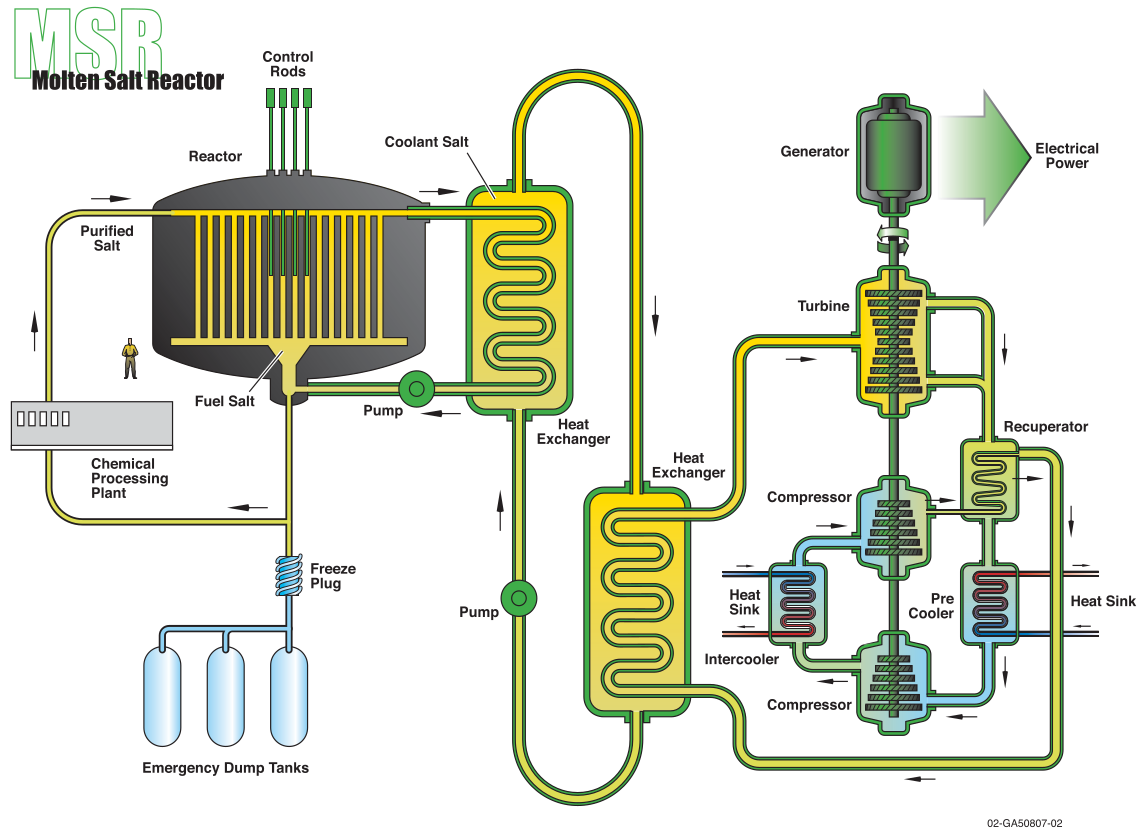
\includegraphics[width=.7\columnwidth]{msr}
	\caption{Schematic diagram of the \gls{MSR} concept. Retrieved from
	\cite{doe_technology_2002}.}
	\label{fig:msr}
\end{figure}

The \gls{MSR} is one of six advanced reactor designs selected at the \gls{GIF} for improved safety,
sustainability, efficiency, and cost over the current generation of predominantly \glspl{LWR}.
Due to the high thermal expansion coefficient, \glspl{MSR} possess an inherently robust
safety feature in the strong negative fuel temperature coefficient of
reactivity \cite{elsheikh_safety_2013}. This reactivity coefficient limits the
maximum temperature that the reactor core would experience in an accident
scenario such as an unprotected reactivity insertion because the subsequent
rise in core temperatures induces a significant drop in reactivity which
quickly neutralizes the initial reactivity insertion. \glspl{MSR} also
operate at a large thermal margin to boiling and can rely on natural
circulation in the event of a pump failure. As a last resort, many \gls{MSR}
designs incorporate a drain plug consisting of actively-cooled frozen salt, which
melts when the core temperatures exceed safety thresholds. The hot molten salt
in the core would then flow down into a drain tank designed to hold the fuel salt in
a subcritical configuration to disrupt any further chain fission reactions.

Some \glspl{MSR} like the \gls{MSBR} or the \gls{MSFR} can
incorporate the thorium fuel cycle for improved sustainability arising from the
use of abundant natural thorium resources and reduced transuranic waste
\cite{heuer_towards_2014}. The latter consequence also reduces costs
associated with long-term nuclear waste storage. In addition, the ability to
operate near atmospheric pressures eliminates the need for a thick pressure
vessel and drives down construction costs, while online fuel reprocessing
reduces reactor downtime during reactor operation \cite{dolan_1_2017}.
We can make further economic arguments supporting \glspl{MSR} in the context of the
carbon-constrained future envisioned in \gls{IEA}'s \gls{NZE} roadmap
\cite{iea_net_2021}. The roadmap for minimizing carbon emissions requires solar \gls{PV}- and
wind-dominated energy markets, which can bring about highly variable electricity generation. The
resulting volatility in electricity prices
encourages the construction of heat storage and peak power
production plants. At the same time, demand for carbon-neutral
fuel will rise as electrification is economically unfeasible
for some industries such as the aviation and marine sectors, which depend on
energy-dense fuels for propulsion. As described by Forsberg
\cite{forsberg_market_2020}, the most cost-efficient options for the
aforementioned resources (heat storage, peak power
production, and hydrogen fuel) all require high-temperature heat.
This requirement favors \glspl{MSR} which are expected to deliver heat at higher average
temperatures than \glspl{LWR} and other high-temperature advanced reactors.
\glspl{MSR} may also possess an edge over other high-temperature advanced reactors from
synergistic benefits of siting molten salt heat storage facilities near the power generation
facility.

\subsection{Past \& Present \gls{MSR} Research \& Development}

\gls{ORNL} researchers first conceived the \gls{MSR} concept in pursuit of a high-temperature
liquid fuel reactor for the US Aircraft Nuclear Propulsion program in
the 1950s \cite{rosenthal_molten-salt_1970}. They
built the first ever operational \gls{MSR}, the 2.5 MW$_{\text{th}}$
\gls{ARE} reactor at \gls{ORNL}. The successful demonstration of the \gls{ARE} spurred further
research into adapting \glspl{MSR} for civilian power generation
\cite{rosenthal_molten-salt_1970}. Continued \gls{MSR} research efforts culminated in the design,
construction, and successful operation of the 8-MW$_{\text{th}}$, thermal-spectrum \gls{MSRE} with
graphite channels and a LiF-BeF$_2$-ZrF$_4$-UF$_4$ fuel salt mixture
\cite{haubenreich_experience_1970}. In addition to other operational achievements, the
\gls{MSRE} became the first reactor to run on $^{233}$U fuel bred from $^{232}$Th. Building on
their experience with the \gls{MSRE}, \gls{ORNL} proposed a new program for the construction and
opeartion of a demonstration reactor based on the \gls{MSBR} concept that they had developed
\cite{macpherson_molten_1985}. The \gls{MSBR} is a thermal-spectrum \gls{MSR} with fertile
$^{232}$Th isotopes mixed directly into the \gls{FLiBe} molten salt for $^{233}$U breeding. Like
the \gls{MSRE}, the \gls{MSBR} was to rely on continuous online salt reprocessing to add fertile
material and remove fission product neutron poisons.
However, the \gls{MSBR} project was canceled prior to the demonstration stage in
favor of the \gls{LMFBR}, which had benefited from a head start in development and stronger
political backing \cite{macpherson_molten_1985}.

Following a relative lull lasting until the late 1990s, renewed research efforts and the \gls{GIF}
provided new impetus for \gls{MSR} research and development. As of the end of 2022, numerous
\gls{MSR} designs exist at various stages of development. Leading \gls{MSR} designs, in terms of
development, licensing, and/or demonstration, include the \gls{MSFR} \cite{merle_optimized_2007},
\gls{MCFR} \cite{terrapower_terrapower_2021}, TMSR-LF1 \cite{zhang_review_2018}, and \gls{IMSR}
\cite{leblanc_18_2017}. The \gls{MSFR} is a fast-spectrum breeder reactor developed through
collaborative efforts from European institutes with funding support from the
European Union. Figure \ref{fig:msfr} shows a schematic diagram of the \gls{MSFR}. As opposed to
the multi-channel design of the \gls{MSRE} and \gls{MSBR}, the
\gls{MSFR} core consists of a large molten salt pool without graphite moderators to avoid
frequent graphite replacements and positive graphite temperature reactivity feedback. The
\gls{MCFR} is a similar pool-type reactor under active development at TerraPower. TerraPower and
Southern Company embarked on a joint project to design, construct, and operate a prototype
\gls{MCRE} design with funding support from \gls{DOE}'s \gls{ARDP}. \gls{CAS} launched the
\gls{TMSR} program in 2011 to develop and construct both solid-fueled and liquid-fueled \gls{TMSR}
designs \cite{zou_research_2019}. They finished construction of TMSR-LF1, a 2-MW$_{\text{th}}$
liquid-fueled prototype, in August 2021 and received approval for reactor commissioning in August
2022. Lastly, Canada-based Terrestrial Energy is also developing their \gls{IMSR}, a small modular
\gls{MSR} based on the \gls{MSRE}, which passed a joint technical review carried out by the
Canadian and US nuclear regulators in July 2022.
%
\begin{figure}[htb!]
	\centering
	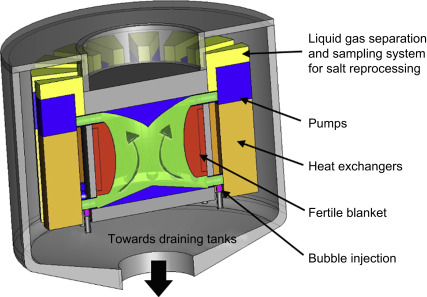
\includegraphics[width=.7\columnwidth]{msfr}
	\caption{Schematic diagram of the \gls{MSFR}. Retrieved from 
	\cite{allibert_7_2016}.}
	\label{fig:msfr}
\end{figure}

\subsection{\gls{MSR} Modeling \& Simulation}

With the renewed global interest in \glspl{MSR}, \gls{MSR} modeling software play an important role
in supporting \gls{MSR} development.
Accurate reactor modeling capabilities are important because they
accelerate reactor design and optimization by enabling quicker iteration through numerous design
changes. \gls{MSR} modeling software are also essential tools in reactor safety analysis and
licensing efforts as reactor developers must demonstrate and verify the \gls{MSR} systems perform
as designed and remain safe under various accident scenarios.

While modeling \glspl{MSR} is not necessarily more difficult than modeling
solid-fueled reactors, we must adapt our software tools to accurately model the
unique phenomena found in these circulating-fuel reactors. The differences in
the challenges of simulating \glspl{MSR} compared to solid-fueled reactors stem
mainly from the liquid fuel form of the fuel salt \cite{diamond_phenomena_2018,
huff_identifying_2019}.

Liquids generally exhibit greater thermal
expansion per unit change in temperature than solids. A decrease in density of
the fuel medium increases the likelihood of neutrons escaping the fuel region
and being absorbed by non-fissile material elsewhere in the reactor.
Consequently, combined with the temperature-dependent Doppler broadening of
resonance capture cross sections, \glspl{MSR} possess stronger negative fuel
temperature reactivity feedback than their solid-fueled counterparts
\cite{elsheikh_safety_2013}. These
phenomena ultimately result in strong interactions between the neutron fluxes
and core temperatures given that neutron fluxes affect core temperatures
through fission heat generation and core temperatures in turn affect neutron
fluxes through the mechanisms as described prior.

With the fuel
salt also serving the role of providing cooling in the core, velocity flow
profiles in the fuel salts strongly impact the temperature distribution via
advection-dominated heat transfer \cite{diamond_phenomena_2018}. This contrasts
with the relatively static temperature profiles in fuel pins and
other forms of solid fuel matrixes, which are physically separate from the coolant.

\glspl{DNP} flow freely within the primary coolant loop as opposed to
being held in place as in solid-fueled reactors. Thus, the delayed neutron
source distribution varies significantly depending on the flow profile and
velocity. In addition, the reactor loses some delayed neutrons from out-of-core
\gls{DNP} decay. These delayed neutrons are considered lost as they're emitted
in subcritical regions and are unlikely to contribute to further fission
reactions in the active core. The reduced delayed neutron fraction in the core
contributes to a greater prompt power spike following a reactivity insertion
event compared to solid-fueled reactors, absent any temperature reactivity
feedback.

Molten-salt flow along various parts of the coolant loop may fall within the turbulent flow
regime, characterized by chaotic eddies, vortices, and other flow instabilities.
Turbulent flow effects further complicate multiphysics interactions of flow with the temperature
and \gls{DNP} distribution. Turbulent flow effects contribute significantly to advection-dominated
heat and particle transfer in molten salt systems, thereby causing enhanced mixing. Therefore,
multiphysics software for \gls{MSR} analysis require adequate flow modeling capabilities with
support for \gls{DNP} drift and some form of turbulence modeling.

\subsection{Moltres for Multiphysics \gls{MSR} Analysis}

Moltres \cite{lindsay_moltres_2017} is an open-source multiphysics reactor simulation software
developed specifically with the considerations for \gls{MSR} characteristics in mind. Moltres is
built on the \gls{MOOSE} \cite{permann_moose_2020} open-source finite-element framework,
which facilitates multiphysics coupling between different
\gls{MOOSE}-based and \gls{MOOSE}-wrapped applications. The \gls{MOOSE} framework also provides
Moltres with advanced meshing and numerical solver capabilities through interfacing with libMesh
\cite{kirk_libmesh_2006} and PETSc \cite{satish_petsc_2019} open-source libraries. Therefore,
Moltres supports up to 3-D unstructured meshes, scales well on high-performance computing systems,
and provides a flexible multiphysics coupling system, which can be tailored for the type of
system being analyzed.

Moltres models coupled neutronics and thermal-hydraulics in reactors. While
generally applicable to most reactor concepts, much of
Moltres' development focuses on meeting the needs of \gls{MSR} multiphysics simulations.
Together with \gls{MOOSE}'s \texttt{Heat}
\texttt{Conduction} and \texttt{Navier-Stokes} \cite{peterson_overview_2018}
modules, Moltres solves the multigroup neutron diffusion
equations, for an arbitrary number of energy and precursor groups, and
thermal-hydraulics equations simultaneously on the same mesh (or separately solved and coupled
through fixed-point iterations if desired).

Lindsay et al. \cite{lindsay_introduction_2018}
demonstrated Moltres' multiphysics \gls{MSR} modeling capabilities with 1D salt
flow in 2D-axisymmetric and 3D models of the \gls{MSRE}. The neutron flux and
temperature distributions agreed qualitatively with legacy
\gls{MSRE} data albeit with some minor quantitative discrepancies due to
simplifications and assumptions in the reactor geometry. I demonstrated Moltres' capabilities for
1) looping of \gls{DNP} drift back into the reactor core, 2) coupling the \gls{DNP}
drift to numerically calculated salt flow profiles within the reactor core,
and 3) a decay heat model to simulate decay heat from fission products, with a 2-D axisymmetric
design of the \gls{MSFR} in my Master's thesis \cite{park_advancement_2020}.

While the Moltres
model of the \gls{MSFR} showed good agreement with other studies in most steady-state and transient
simulation cases, the Moltres model showed significant discrepancies during pump-initiated
transient scenarios in the absence of a proper turbulence model. Instead, the model applied a
uniform eddy viscosity assumption, which proved to be inadequate under non-steady flow. In order to
advance Moltres as a multiphysics simulation software for \gls{MSR} analysis, Moltres requires a
turbulence modeling capability to capture adequate turbulent flow phenomena and its interactions
with other physics present in \glspl{MSR}.

\subsection{\gls{VV} of Multiphysics \gls{MSR} Models and Software}

\gls{VV} of simulation software and models are important steps in simulation software development
\cite{sargent_verification_2010}. Verification is the process of checking whether a software
and its implementation accurately represents the conceptual description and specifications.
Validation is the process of checking whether a model is an accurate representations of the real
world within the range of its intended uses. For reactor software, verification is commonly
performed by comparison with other reactor software designed to run the same type of reactor
simulations. On the other hand, validation is performed by comparing numerical results from
a simulation model to experimental data from the corresponding live test. The validity of a model,
and the results derived from it, depends on the outcome of both verification and validation.

The important multiphysics phenomena in \glspl{MSR} for \gls{VV} are salt flow-induced
\gls{DNP} drift and the strong coupling between neutron flux and temperature advection-diffusion.
Notable \gls{VV} studies on \gls{MSR} modeling include work by Delpech et al.
\cite{delpech_benchmark_2003}, Tiberga et al. \cite{tiberga_results_2020}, Fratoni et al.
\cite{fratoni_molten_2020}, and Brovchenko et al. \cite{brovchenko_neutronic_2019} in relation to
the \gls{MSRE} and the \gls{MSFR} designs.



Delpech et al. \cite{delpech_benchmark_2003}
published one of the first modern \gls{VV} work for \gls{MSR} multiphysics modeling. Collaborators
from six institutions modeled \gls{MSRE} pump start-up, pump coast-down, and natural
circulation transients to assess and validate their models and codes for studying the effects of
salt flow on the reactivity and power. Given the wide range of neutronics methods from
multidimensional Monte Carlo methods to zero-dimensional point reactor kinetics, some deviations
were observed between different codes. Neverthless, all results showed generally good agreement
with \gls{MSRE} experimental data from \gls{ORNL}.

As mentioned in Subsection \ref{sec:msr-tools}, Tiberga et al. \cite{tiberga_results_2020}
published the CNRS benchmark for the verification of \gls{MSR} simulation tools designed for
fast-spectrum \gls{MSR} modeling. In contrast with the multi-channel \gls{MSRE} and its derivative
designs, the CNRS benchmark has a 2 m$\times$2 m problem domain of homogeneous fuel salt mimicking
the large salt pool in fast-spectrum \gls{MSR} designs. The CNRS benchmark consists of three phases
starting with single-physics calculations in Phase 0, followed by problems which gradually
introduce multiphysics coupling in Phase 1, and lastly time-dependent pertubation problems in Phase
2. Thus, the benchmark provides a systematic approach aimed towards helping code developers
identify sources of discrepancies which may otherwise be masked by error cancellation or other
dominant sources of discrepancies. The final steady-state and time-dependent problems involve
studying the effects of natural circulation and lid-driven flow on the reactivity and power output.
Aside from the problem specifications, Tiberga et al. also published the associated group
constant cross section data required by deterministic neutronics solvers to perform neutronics
calculations. Four institutions participated in the benchmarking exercise with neutron diffusion,
$SP_N$, and $S_N$-based solvers for the neutronics calculations. Their measured neutronics and
\gls{TH} parameters showed excellent agreement within up to 2.5\% discrepancy from their combined
average.

Neutronic benchmark studies of the \gls{MSRE} and the \gls{MSFR} by Fratoni et al.
\cite{fratoni_molten_2020} and Brovchenko et al. \cite{brovchenko_neutronic_2019} measured the
delayed neutron losses due to the decay of \glspl{DNP} flowing out of the active core region.
Fratoni et al. sought to establish a standard validation platform for \gls{MSR} neutronics
simulation tools with \gls{MSRE} experimental data for inclusion in the \gls{IRPhEP} handbook.
They characterized and validated a model of the \gls{MSRE} in the Monte Carlo particle transport
code Serpent. On the other hand, the \gls{MSFR} benchmark by Brovchenko et al. featured results
from multiple \gls{MSR} simulation tools by several collaborators. Their assessment found that
the choice of nuclear database for the cross sections and decay data has the most significant
impact on the neutronics results.

While these publications have plugged significant technical gaps, more can be done to develop
open \gls{VV} procedures for \gls{MSR} multiphysics modeling. For instance, the
CNRS benchmark does not assess the loss of delayed neutrons due to the decay of \glspl{DNP} flowing
out of the active core region. This phenomenon is important as the delayed neutron fraction in the
core directly impacts the transient power response in unprotected accident scenarios. Meanwhile,
the neutronic benchmark studies by Fratoni et al. \cite{fratoni_molten_2020} and Brovchenko et al.
\cite{brovchenko_neutronic_2019} did not provide standardized group constant data required by most
deterministic multiphysics \gls{MSR} simulation tools. Therefore, it is difficult to isolate
discrepancies arising from code implementations as opposed to discrepancies from using different
nuclear databases or stochastic uncertainties in Monte Carlo simulations. A good model verification
procedure for delayed neutron loss should ideally provide well-defined problems and the necessary
input data. It is also helpful to perform model verification studies on simpler problems like the
bare homogeneous problem domain in the CNRS benchmark before embarking on more complicated
validation studies which require accurate models of the reference experiments.

\section{Objectives}

This thesis demonstrates latest capabilities of Moltres
\cite{lindsay_introduction_2018}.
In particular, this thesis presents two more recent
developments in Moltres, namely fully integrating \gls{MOOSE}'s incompressible
Navier-Stokes module into Moltres, and introducing a
decay heat model.
The main objective of this thesis is to verify Moltres'
latest capabilities in modeling multiphysics, steady-state, and transient
behavior of fast-spectrum \glspl{MSR} through the study of the \gls{MSFR}
concept. Code-to-code verification is an important exercise in software
development for ensuring that the application produces accurate and reliable
results. This thesis covers the \gls{MSFR} concept mainly because it has been
studied extensively with readily available data in the literature to verify
against. The \gls{MSFR} design also features interesting flow
patterns that greatly affect the steady-state and transient behavior. This
present work will first present a verification of Moltres' \gls{MSFR}
diffusion neutronics against the Monte Carlo neutron transport software
Serpent 2, followed by a verification of
the coupled neutronics/thermal-hydraulics steady-state and accident transient
results against two sets of results published by
Fiorina et al. \cite{fiorina_modelling_2014}. The two sets of results arose
from a collaborative benchmarking exercise by researchers at Politecnico di
Milano and Technical University of Delft with two separate \gls{MSR}
simulation tools. Section \ref{chap:lit} discusses these tools
in greater detail. The
secondary objective is to identify areas of improvement in Moltres for future
development.

\section{Outline}

The outline of this thesis is as follows. Chapter 2 discusses the history and
features of \glspl{MSR}, and a literature review of existing \gls{MSR}
simulation tools. The chapter also covers the \gls{MSFR} concept in greater
detail. Chapter 3 details the software and the general modeling
approach for generating the results in this thesis. Chapter 4 provides a
neutronics assessment by comparing key neutronics parameters from Moltres'
eigenvalue calculations to Serpent's Monte Carlo calculations. Chapter 5
presents steady-state results of coupled neutronics/thermal-hydraulics
\gls{MSFR} simulations in Moltres. Chapter 6 presents accident transient
simulation results for unprotected reactivity insertions, unprotected loss of
heat sink, unprotected loss of flow, and unprotected pump overspeed. Lastly,
Chapter 7 summarizes the key findings in this thesis
and posits some potential avenues for future work.
